%% ========================================================================
%%							K-Means
%% ========================================================================


\chapter{$k$-means}
\label{cha:K-means}

To be able to process, summarize and understand huge amounts of data better, one is interested in methods that are able to find patterns in the data. The characteristics of these patterns then can be represented by just a few representative data points which behave like the whole data set. Given a  data set the challenge is, based on a measure of similarity, to find groups of observations which are quite similar within each group but quite different to all the other groups. If this task has to be done with unlabeled data it is referred to as unsupervised clustering (c.f.\cite{jain2010data}). One of the most widely used unsupervised clustering approaches is the $k$-means clustering. The $k$-means method is a simple approach in cluster analysis which splits a data set of $n$ $p$-dimensional observations into $k$ distinct clusters. Each observation belongs uniquely to exactly one of the $k$ clusters, where $k$ is a predefined number of clusters. Let $C=\{C_1, C_2 \dots, C_k\}$ denote the sets containing the indices of the observations  related to the clusters, then we get:
\begin{definition}
Let $X=\{x_1, ..., x_n\}$ be a data set. X is said to be partitioned into $k$ different clusters $C_1, C_2 \dots, C_k$ if
	\begin{enumerate}[label=(\roman*)] \centering
		\item $C = C_1 \cup C_2 \dots \cup C_k = \{1, \dots, n\}$

		\item $C_i \cap C_j = \emptyset \quad \forall i \neq j$
	\end{enumerate}
\end{definition}
The basic idea of the $k$-means clustering is to minimize the variation within the clusters. For this purpose some distance measure is needed in order to be able to define variation within clusters.
\begin{definition}\label{def:metric} Let X be a set, d: X$\times$X $\rightarrow~\R$ a function. Then d is called a metric (or distance) on X if for all x, y, z $\in$ X the following conditions are fulfilled: 
\begin{enumerate}[label=(\subscript{D}{\arabic*})]
	\item\label{itm:namee} $d(x,y) = 0 \Leftrightarrow x = y$ \hfill (Identity of indiscernibles)
	\item $d(x,y) = d(y,x)$  \hfill (symmetry)
	\item $d(x,z) \leq d(x,y) + d(y,z)$ \hfill (triangle inequality)
\end{enumerate}

\begin{remark}
	Given the axioms from definition \ref{def:metric} it can be shown that a non-necgativity property can be deducted e.g. $d(x,y) \geq 0 ~\forall x,y \in X$.
	\begin{equation*}
	\begin{split}
		d(x,y) + d(y,x) & \geq d(x,x) \\
		d(x,y) + d(x,y) & \geq d(x,x) \\
		2d(x,y)         & \geq 0      \\
		d(x,y)          & \geq 0      \\
	\end{split}
	\end{equation*}
	%%	\item $d(x,y) \geq 0$ \quad (non-negativity) 
\end{remark}


\begin{example}(c.f. \cite{analysis_1}) The most common used distance functions for two points $x=(x_1, ..., x_p)$ and  $y=(y_1, ..., y_p)$ in $\R^p$ are: 
	\begin{itemize}[label=$\star$]
		\item Euclidean distance:
			\begin{equation*}
				d_2(x,y) := \sqrt{\sum_{j=1}^p(x_j - y_j)^2}
			\end{equation*}
		\item Manhattan distance:
			\begin{equation*}
				d_1(x,y) := \sum_{j=1}^p|x_j - y_j|
			\end{equation*}
		\item Chebyshev (maximum) distance:
			\begin{equation*}
				d_\infty(x,y) := \max_j|x_j - y_j|
			\end{equation*}		
		\item Minkowski distance ($L^q$ distance) with q $\geq$ 1:
			\begin{equation*}
				d_p(x,y) := \bigg(\sum_{j=1}^p(x_j - y_j)^q\bigg)^{\frac{1}{q}}
			\end{equation*}	
	\end{itemize}
\end{example}

\end{definition}
Typically the Euclidean distance is used as a measure of similarity to compute the distance between the different points. By using the Euclidean metric as a measure of similarity one assumes that the clusters are spherical. 
\begin{definition}
	 Let the Euclidean metric be the measure of similarity for the data points in the data set $X=\{x_1, ..., x_n\}$ and p the dimension of the data. Then the variation within one cluster $C_l,~l=1, ..., k$ is defined as:  
	\begin{equation*}
		D(C_l) := \frac{1}{|C_l|}\sum_{j=1}^p \sum_{i,i' \in C_l} (x_{ij} - x_{i'j})^2
	\end{equation*}
\end{definition}

\begin{remark} \label{rem:average}
	For the average over one dimension in one cluster we use the short notation
	$\bar x_{lj} = \frac{1}{|C_l|} \sum_{i \in C_l} x_{ij}$.
\end{remark}

\begin{remark} \label{rem:identity}
 	The identity $\sum_{i \in C_l}(x_{ij}-\bar x_{lj})^2 = \big( \sum_{i \in C_l} x_{ij}^2 \big) - |C_l| \bar x_{lj}^2$ can be verified by simple calculus. 
\end{remark}

\begin{corollary}\label{equ:Steiner}
The variation within one cluster, $D(C_l)$ can be written as: 
	\begin{equation}
		D(C_l) =2 \sum_{i \in C_l} \sum_{j=1}^p (x_{ij}-\bar x_{lj})^2
	\end{equation}
\end{corollary}
\begin{proof}
	\begin{equation*}
	\begin{split} %% used to get only one number for all lines instead of one number per line
		D(C_l)	&= \frac{1}{|C_l|}\sum_{j=1}^p \sum_{i,i' \in C_l} (x_{ij} - x_{i'j})^2 \\
				&= \frac{1}{|C_l|}\sum_{j=1}^p \sum_{i,i' \in C_l} x_{ij}^2 - 2x_{ij} x_{i'j} + x_{i'j}^2 \\
				&= \sum_{j=1}^p \Bigg( \frac{1}{|C_l|} \sum_{i,i' \in C_l} x_{ij}^2 - 2 \frac{1}{|C_l|} \sum_{i,i' \in C_l} x_{ij} x_{i'j} + \frac{1}{|C_l|} \sum_{i,i' \in C_l} x_{i'j}^2 \Bigg) \\
				& \overset{(Remark~\ref{rem:average})}{=} \sum_{j=1}^p \Bigg( \sum_{i \in C_l} x_{ij}^2 - 2 \bar x_{lj} \sum_{i \in C_l} x_{ij} + \sum_{i' \in C_l} x_{i'j}^2 \Bigg) \\
				& \overset{(Remark~\ref{rem:average})}{=}2 \sum_{j=1}^p \Bigg( \sum_{i \in C_l} x_{ij}^2 - |C_l| \bar x_{lj}^2 \Bigg) \\
				& \overset{(Remark~\ref{rem:identity})}{=} 2 \sum_{i \in C_l} \sum_{j=1}^p (x_{ij}-\bar x_{lj})^2
	\end{split}
	\end{equation*}
\end{proof}

The approach of $k$-means is to find a partitioning of the data set in such a way that the sum of the variations is minimized.

\begin{definition}[$k$-means]
Let $X = \{x_1, ..., x_n\}$ be a data set and $\{C_1, ..., C_k\}$ a partition. Then $k$-means tries to find an optimal partition $C^* = \{C_1^*, ..., C_k^*\}$ such that: 
	\begin{equation}\label{equ:K-means}
		\sum_{l=1}^k D(C_l^*) = \underset{C_1, \dots, C_k}{\text{min}} \sum_{l=1}^k D(C_l) = \underset{C_1, \dots, C_k}{\text{min}} ~2 \sum_{l=1}^k  \sum_{i \in C_l} \sum_{j=1}^p (x_{ij}- \bar x_{lj})^2
	\end{equation}
\end{definition}

When it comes to solving the optimization problem defined by formula (\ref{equ:K-means}), the computational complexity of the algorithm to be used is of high interest. Therefore computational complexity theory categorizes problems into different classes that have some defining properties, one of which is called NP-hard. The definition of these classes would go beyond the scope of this work and therefore only a reference to the literature is given here e.g. \cite{np_hard_reference}. In very simplified terms one can say that there are currently no efficient algorithms for this type of problem. 


\begin{corollary}
	Solving the $k$-means problem defined in (\ref{equ:K-means}) is NP-hard.
\end{corollary}
\begin{proof}
c.f. \cite{NP_hard}
\end{proof}

Even though the problem is NP-hard it is still possible to provide algorithms which converge to a local optimum. The algorithms used for finding a local minimum work on an iterative basis   and involve just a few different steps. The $k$-means algorithms either start with an initial assignment of all observations to $k$ different clusters or with $k$ distinctly selected cluster centers. The next step is to find a new cluster center such that the variation $D(C_l)$ is minimized within each cluster. Then all data points $X = \{x_1, ..., x_n\}$ are reassigned to the cluster which is nearest and the minimization procedure is repeated until convergence. 

\begin{remark}~	
	\begin{enumerate}[label=(\roman*)]
		\item  For $k=n$, (\ref{equ:K-means}) is zero because each data point represents a cluster. 
	\end{enumerate}
\end{remark}

One possible formulation for an algorithm that converges to a local optimum is the one from Lloyd \cite{lloyd1982least} which a pseudo code is given below. Note that for algorithm \ref{alg:K-means} we have a fixed number of clusters $k$ as well as a finite set of possible partitions $k^n$. We can therefore show that the stated algorithm converges to a local minimum by minimizing (\ref{equ:Steiner}).

\begin{remark}~
	\begin{enumerate}[label=(\roman*)]
		\item For any set of observations S it holds that: 
			\begin{equation*}
				\bar x_S = \underset{x}{\text{argmin}}\sum_{i \in S} (x_i - x)^2
			\end{equation*}
			Hence, step \ref{lev:K-means_two}\ref{lev:K-means_two_a} minimizes the sum of squared deviations and therefore $D(C_l)$.
		\item Step \ref{lev:K-means_two}\ref{lev:K-means_two_b} which reassigns the observations to the new nearest centroid can only reduce the objective function.
	\end{enumerate}
\end{remark}

	
\begin{algorithm}
	\caption{$k$-means clustering \cite{Introducion_Stat_Learning} - Lloyd's algorithm}\label{alg:K-means}
\begin{algorithmic}
\\
	\begin{enumerate}
	\item Choose $k$ initial centroids randomly.
	\item  \label{lev:K-means_two}Iterate till the cluster assignments stop changing:
	\begin{enumerate}[label=\emph{\alph*})]
		\item \label{lev:K-means_two_a} For each of the $k$ clusters, compute the cluster centroid. The $i$-th cluster centroid is the vector of the $p$ parameter means for the observations in the $i$th cluster. 
		\item \label{lev:K-means_two_b}Assign each observation to the cluster whose centroid is closest in the sense of Euclidean distance. 
	\end{enumerate}
	\end{enumerate}
\end{algorithmic}
\end{algorithm}

%\break
\begin{remark}~
	\begin{enumerate}[label=(\roman*)]
		\item The $k$-means algorithm always converges and finds a local optimum which need not to be the global one.
		\item Different clustering results can be obtained when different initial cluster assignments in step 1 of algorithm \ref{alg:K-means} are chosen.
	\end{enumerate}
\end{remark}

\begin{remark}[Running Time]~
	\begin{enumerate}[label=(\roman*)]
		\item Algortihm \ref{alg:K-means} has a running time of $O(nkpi)$, with n being the number of data points, k the number of cluster, p the number of dimensions and i the number of iterations needed to converge. The only unknown variable is the number of iterations. 
		\item The trivial upper bound for the number of iterations needed is given by $O(k^n)$, because the algorithm visits every partition of points only once. 
		\item It can be shown \cite{arthur2006slow} that in the worst case scenario the running time of the algorithm is superpolynomial with a lower bound for the number of iterations of $O(2^{\Omega(\sqrt{n})})$. That means that the running time cannot be bounded above by any polynomial function.
		\item In practice, the number of iterations required is often small, which makes the algorithm appear to be linearly complex.  
	\end{enumerate}
\end{remark}

It is advisable to run the algorithm several times with different initial centroid assignments. This increases the likelihood of finding a partition that is close to the optimum and thus provides a low value for the objective function (\ref{equ:K-means}). However, the biggest challenge when using $k$-means is the estimation of the optimal number of clusters $k$. Figure (\ref{fig:cluster_centers}) shows an example with three clusters that illustrates the different clustering results when the number of $k$  increases. Panel (a) shows the raw data with three clusters ($k_{true} = 3$), each generated by an uniform distribution. Panels (b), (c) and (d) show the cluster results with $k = 2, 3 $ and $7$, respectively. If the number of clusters $k$ is smaller than the actual number of clusters in the data, then $k$-means merges clusters, while for $k$ greater than $k_{true}$, $k$-means divides well seperated clusters. Panel (b) shows a merge of the clusters at the top right, whereas panel (d) shows an artificial split of two natural clusters for $k=5$. For the grouping of similar data points and their representation by a cluster center, an underestimation of the actual number of clusters is more critical than an overestimation. If $k$ underestimates the true value of clusters ($k < k_{true}$), then it's  not possible to capture the cluster specific characteristics for the merged clusters because they are represented by only one cluster center. However, an overestimation of $k_{true}$ is not so critical because some natural clusters will be represented by two cluster centers which has a negative impact on the compression ratio but not the clustering quality. For the most crucial step of $k$-means, a comprehensive collection of methods for estimating the correct number of clusters can be found in \cite{milligan1985examination}. In the following, the `elbow' and silhouette method, two widely used graphical methods for estimating $k_{true}$, are presented and applied to the sample data set. 
\begin{figure}
	\centering
	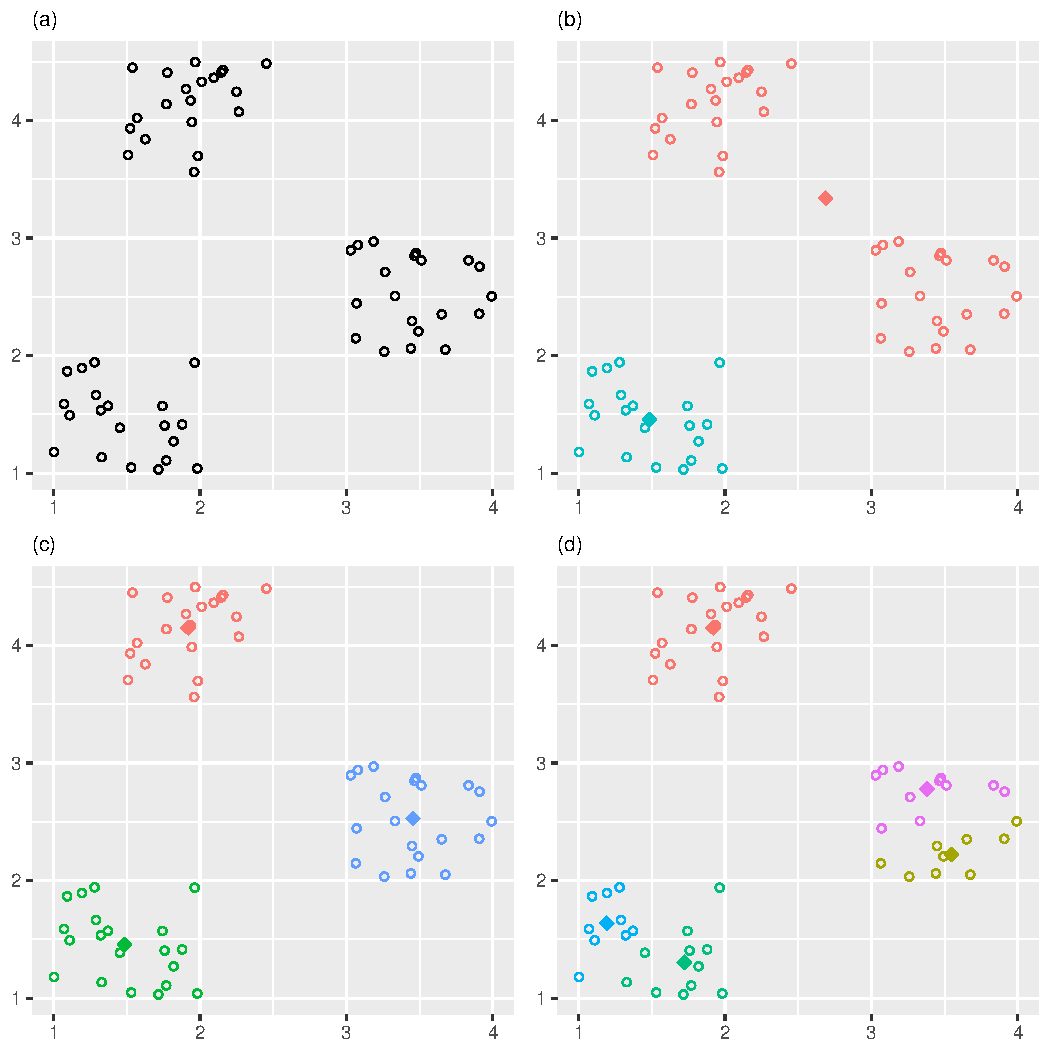
\includegraphics[width=0.8\textwidth]{figures/chapter_k_means/cluster_centers}
	\caption{Results for a three-cluster example: (a) raw data; (b) $k=2$; (c) $k=3$; (d) $k=5$}
	\label{fig:cluster_centers}
\end{figure}


\clearpage % ensure that all stuff is plotted (images)
%%%---------------------------------------------------------------------------------------------------------------------
%%%			Elbow method
%%%---------------------------------------------------------------------------------------------------------------------
\section{Elbow method - gap statistic}
Estimating $k$, the parameter that defines the number of clusters, is one of the most difficult  tasks when using k-means. While it is still possible to graphically determine the number of clusters by plotting the data in 2 or 3 dimensional spaces, other methods must be used in higher dimensions. The `elbow' method is one of the most commonly used methods in this context. 

\begin{definition}
Let $X = \{x_1, ..., x_n\}$ be a data set and k the number of clusters. Then $C=\{C_1, ..., C_k\}$ is the corresponding partition with the sum of variation within all clusters defined as: 
	\begin{equation*}
		V_k := \sum_{r=1}^k \frac{D(C_r)}{2}
	\end{equation*}
\end{definition}

 Plotting $V_k$, the sum of variation within all clusters as a measure of total error versus the number of clusters used gives a good indication for the true value of $k$. Figure \ref{fig:gap_statistics}(a) shows that the error measure $V_k$ decreases monotonically as the number of clusters increases but there seems to exist a $k$ from which the decline is clearly flattened. Such an `elbow' indicates that any additional cluster reduces the total variation $V_k$ only slightly and an appropriate number of clusters can be derived from the location of the `elbow'. In accordance with $k_{true}=3$, the `elbow' plotted in \ref{fig:gap_statistics}(a) indicates that the true number of clusters is three, because there the curve starts to flatten dramatically. Even if the sample data set consists of very well separated clusters, the example indicates that the method could also be suitable in general use cases. For a small number of tasks the graphical determination of the "elbow" is practicable, but an automated method is needed with an increasing number of clustering operations. A statistical method that formalizes this procedure of finding the `elbow' is described in \cite{tibshirani2001estimating}.
 The basic idea is to make the sum of variation $V_k$ comparable to a reference. For this purpose, the sum of deviations is calculated for each $k$ and then compared with the expected sum of the deviations 
 derived from a reference data set with no obvious clustering. The reference data set is generated by sampling uniformly over the range of the observed values for every feature from the original data set.
 This means it is sampled uniformly from the smallest $p$-dimensional cube that contains all data points $\{x_1, ..., x_n\}$ of the original data set.  
 
\begin{definition}
Let $k$ be the number of clusters and $\E_n$ the expectation under a sample of size $n$ from
the reference distribution. Then the gap-statistic is defined as: 
	\begin{equation}\label{equ:gap_statistic}
		Gap_n(k) := \E_n\big[log(V_k) \big] - log(V_k)
	\end{equation}
\end{definition}

To determine the expected value $\E_n\big[log(V_k) \big]$ we draw $B$ different samples $\{x_1^*, ..., x_n^*\}$ from the $p$-dimensional cube and average over the $B$ values of $log(V_k)$. Accounting for the simulation error introduced by using the $B$ Monte Carlo samples the standard deviation is given by: 

\begin{equation*}
	s_k = \sqrt{1 + \frac{1}{B}} sd(k)
\end{equation*}

The optimal cluster size $k$ is then determined by the following rule which identifies the `elbow':

\begin{definition} Let $Gap(k)$ be the statistic defined above and $s_k$ the standard error (c.f. \cite{tibshirani2001estimating}). Then the rule for choosing $k$ is given by: 
	\begin{equation}\label{equ:gap_statistic_rule}
	\hat{k} := \text{smallest } k \text{ such that } Gap(k) \geq Gap(k+1) - s_{k+1}
	\end{equation}
\end{definition}

In order to find the optimal number of clusters in a computational way, the following steps described in algorithm \ref{alg:ellbow} are necessary:

\begin{algorithm} \label{alg:ellbow}
	\caption{Ellbow method \cite{tibshirani2001estimating}}\label{alg:ellbow}
	\begin{algorithmic}
		\\
		\begin{enumerate}
			\item Define the maximal number of clusters $k_{max}$
			\item Iterate over $k = 1, ..., k_{max}$:
			\begin{enumerate}[label=\emph{\alph*})]
				\item \label{lev:ellbow_a} Apply the $k$-means algorithm to the data set $\{x_1, ..., x_n\}$ and calculate $log(V_k)$.
				\item \label{lev:ellbow_b} Generate $B$ reference data sets, each of them having $n$ samples $\{x_1^*, ..., x_n^*\}$.
				\item \label{lev:ellbow_c} Cluster each of those $B$ data sets and calculate $\E_n\big[log(V_k) \big] = \frac{1}{B} \sum_{b=1}^B log(V_{kb})$ 
				\item \label{lev:ellbow_d} Compute the standard deviation: 
					\begin{equation*}
						sd(k) = \bigg(\frac{1}{B}\sum_{b=1}^B(log(V_{kb})-\E_n\big[log(V_k) \big])^2\bigg)^\frac{1}{2}
					\end{equation*}
				\item \label{lev:ellbow_e} End the loop if: $Gap(k) \geq Gap(k+1) - s_{k+1}$ 
			\end{enumerate}
		\end{enumerate}
	\end{algorithmic}
\end{algorithm}

\begin{figure}
	\centering
	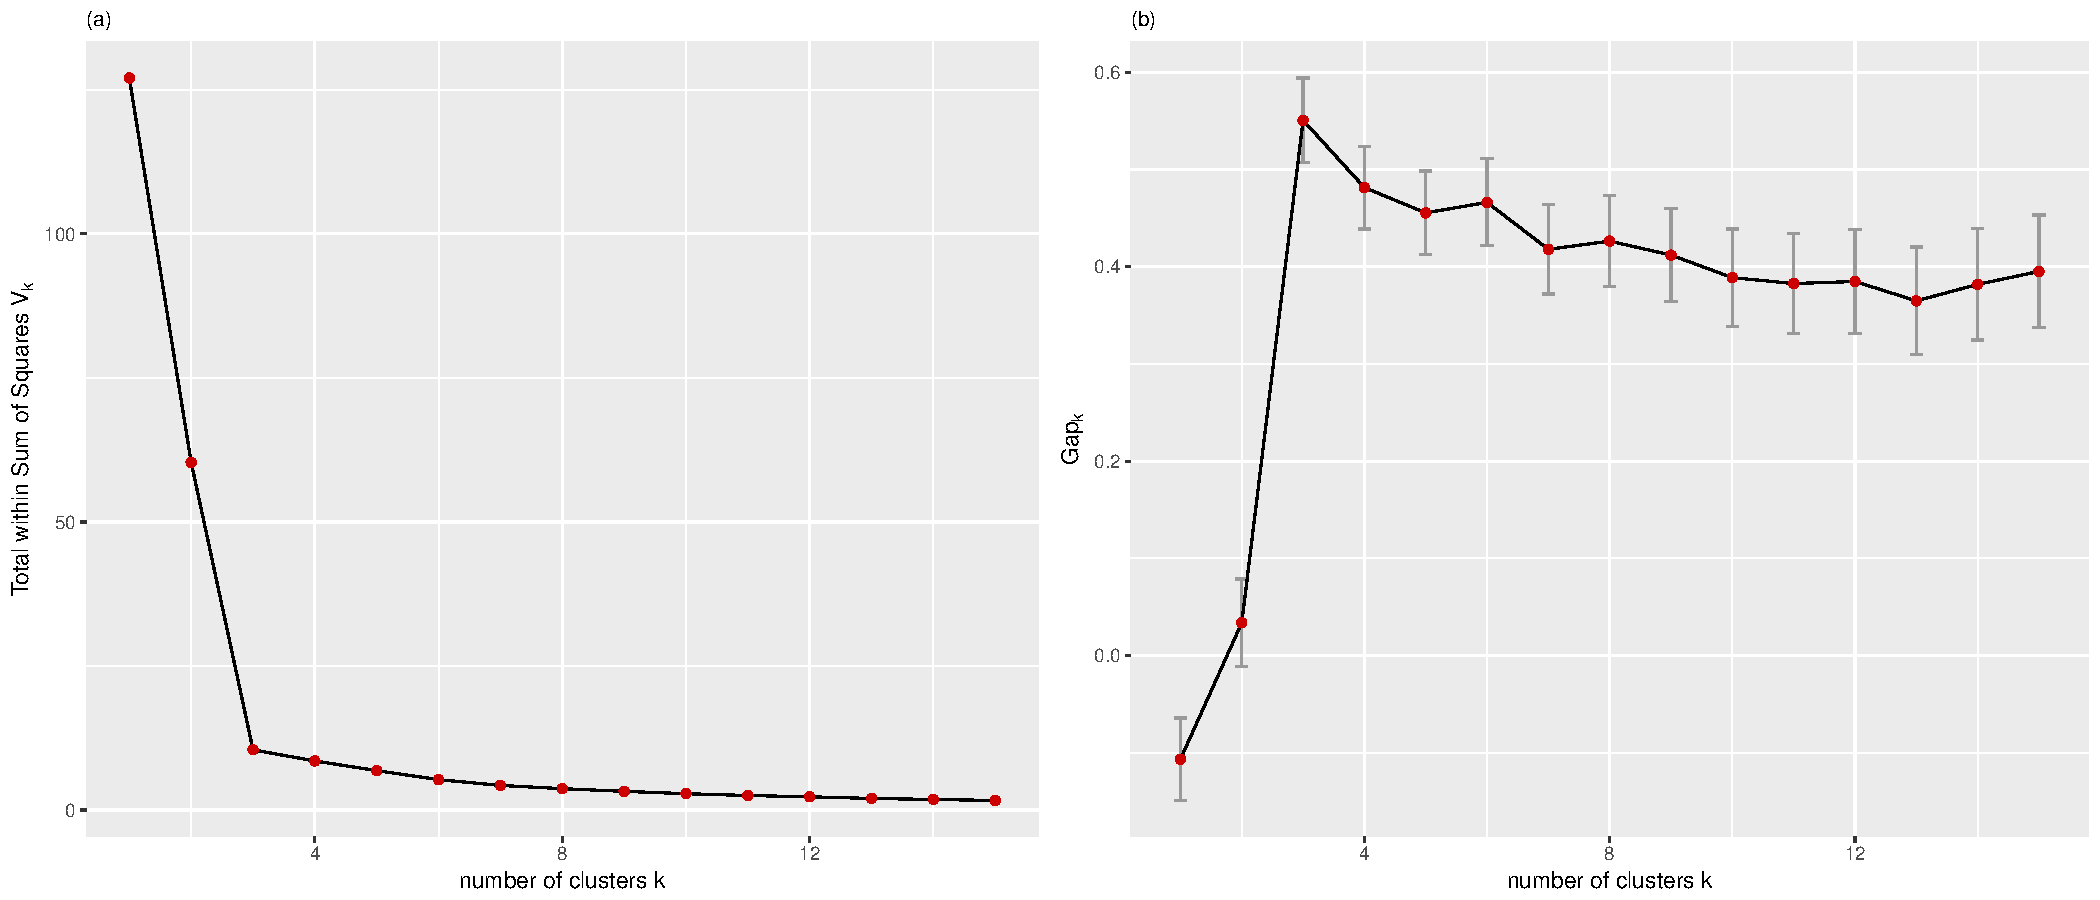
\includegraphics[width=\textwidth]{figures/chapter_k_means/gap_withinSS}
	\caption{Three-cluster example: (a) Total within Sum of Squares; (b) Gap-Statistic}
	\label{fig:gap_statistics}
\end{figure}

Figure (\ref{fig:gap_statistics})(b) shows the gap-statistic for different values of $k$ with the corresponding standard errors as a vertical bar. The application of the proposed rule (\ref{equ:gap_statistic_rule}) for selecting the number of clusters results in $\hat{k} = 3$ which corresponds exactly to the actual number of clusters in the data set. 

%%%---------------------------------------------------------------------------------------------------------------------
%%%			Silhouette method
%%%---------------------------------------------------------------------------------------------------------------------
\section{Silhouette method}\label{sec:silhouette}

Although the "elbow method" is well suited in many cases to determine the number of clusters, the resulting partitioning is not visually displayable if the dimension is larger than three. A visually appealing graphical display called silhouette plot introduced in \cite{rousseeuw1987silhouettes} tries to overcome this shortcoming in order to be able to interpret cluster results more properly. The plot shows whether a specific partitioning result reflects a cluster structure actually present in the data set or not, by comparing the within dissimilarity with the between dissimilarity for every data point. It can thus be determined how similar a data point is to its own cluster compared to the other clusters. The measure of similarity can be calculated with any distance metric appropriate to the specific problem and will be called $dist(x_i, x_j)$ for two data points $x_i$ and $x_j$.

\begin{definition}[Within dissimilarity]
	Let $X=\{x_1, ..., x_n\}$ be a data set and $C=\{C_1, ..., C_k\}$ the corresponding partitioning with $k$ cluster. Assume that the data point $x_i$ is assigned to cluster $C_i$ with $1 \leq i \leq k$. Then the average dissimilarity of $x_i$ to all other objects assigned to cluster $C_i$ is defined by: 
	\begin{equation*}\label{equ:dist_A}
	WD(C_i,i) := \frac{1}{|C_i|}\sum_{x_l \in C_i} dist(x_i, x_l)
	\end{equation*}
\end{definition}

One can think of $WD(C_i,i)$ as a measure of how well the data point $x_i$ is embedded in its cluster $C_i$. The smaller the value, the closer the data points of the cluster are to each other on average. 

\begin{definition}[Between dissimilarity]
	Let $X=\{x_1, ..., x_n\}$ be a data set and $C=\{C_1, ..., C_k\}$ the corresponding partitioning with $k$ cluster. For any cluster $C_{j}$ different from $C_i$ (i.e. $i \neq j$) the average dissimilarity of  $x_i \in C_{i}$ to the cluster $C_{j}$ is given by: 
	\begin{equation*}\label{equ:dist_C}
		BD(C_j,i) := \frac{1}{|C_j|}\sum_{x_l \in C_j} dist(x_i, x_l) 
	\end{equation*}
\end{definition}

One can see that $BD(C_j,i)$ is the average distance from data point $x_i$ in cluster $C_i$ to all data points $x_j$ in cluster $C_j$. 

\begin{definition}
	Let $X=\{x_1, ..., x_n\}$ be a data set and $C=\{C_1, ..., C_k\}$ the corresponding partitioning with $k$ cluster. For any data point $x_i$ assigned to cluster $C_i$ (e.i. $x_i \in C_i$) the distance to the closest neighbor cluster is given by: 
	\begin{equation*}\label{equ:dist_B}
		dist(i) := \min_{C_i\neq C_j} BD(C_j,i)
	\end{equation*}
\end{definition}

Cluster $C_b$ with $1 \leq b \leq k$, which shares the smallest average dissimilarity with point $x_i \in C_i$ is called the neighbor cluster of $x_i$. This neighbor cluster is the first choice if cluster $C_i$ is removed from our analysis and we have to reassign $x_i$ to a new cluster. After computing $WD(C_i,i)$ and $dist(i)$ for every data point $x_i,~i=1,...n$ one can define the silhouette statistic $s(i)$ as follows.

\begin{definition}
Let $X=\{x_1, ..., x_n\}$ be a data set and $C=\{C_1, ..., C_k\}$ the corresponding partitioning with k cluster. For every $x_i \in X$ the silhouette $s(i)$ is defined as:
	\begin{equation*}\label{equ:silhouette_long}
	s(i) = \begin{cases}
		1-\frac{WD(C_i,i)}{dist(i)} 	& \text{ if } WD(C_i,i) < dist(i)\\
		0 								& \text{ if } WD(C_i,i) = dist(i)\\
		\frac{dist(i)}{WD(C_i,i)}-1 	& \text{ if } WD(C_i,i) > dist(i)
	\end{cases}
	\end{equation*}
\end{definition}

\begin{remark}
	We can write the silhouette $s(i)$ in a more compact form: 
	\begin{align*}
		s(i) &= \frac{dist(i) - WD(C_i,i)}{max\{ WD(C_i,i), dist(i) \}},  &\text{ if } |C_i|>1 \\
		s(i) &= 0  &\text{ if } |C_i|=1
	\end{align*}
\end{remark}

\begin{remark}
	For every $x_i$ it is true that $-1 \leq s(i) \leq 1$.
\end{remark}

\begin{remark}
	In order to understand which values of $s(i)$ correspond to which clustering results, it makes sense to look at values at the boundaries: 
	\begin{itemize}[label=$\star$]
		\item $s(i) \in (1 - \epsilon, 1]$: For $s(i)$ close to 1 the within dissimilarity of $x_i$ is much smaller than the minimum between dissimilarity. This shows on the one hand that the data point $x_i$ is very well embedded in its cluster and has a small distance to the other data points of its cluster (i.e. $WD(C_i,i)$ small). On the other hand a relatively large value of $dist(i)$ shows that the minimum distance from $x_i$ to the nearest cluster is very large. Thus one can speak of adequate clustering.		
		\item $s(i) \in (-\epsilon, + \epsilon)$: The within dissimilarity of $x_i$ is approximately the same as the minimum between dissimilarity which indicates that $x_i$ lies between two cluster. A small change of the data point $x_i$ could cause it to be assigned to another cluster, suggesting unstable results.		
		\item $s(i) \in [-1, -1 + \epsilon)$ The minimum between dissimilarity of $x_i$ is much smaller than the within dissimilarity which indicates that $x_i$ may not be correctly clustered. In this case $x_i$ is on average much closer to the neighbor cluster than to the actual cluster which rises doubts if the cluster assignment is right. 
	\end{itemize}
\end{remark}

\begin{remark}	
	Let $x_i$ be a data point which is assigned to cluster $C_i$ and cluster $C_j$ the neighbor cluster of $x_i$. If $x_i$ is reassigned from cluster $C_i$ to cluster $C_j$ then $s (i)$ becomes $-s(i)$
\end{remark}
In order to get a visually appealing overview if a clustering result is good or not all silhouettes are plotted on top of each other. Silhouettes which belong to the same cluster are plotted together and ranked in decreasing order.

\begin{figure}
	\centering
	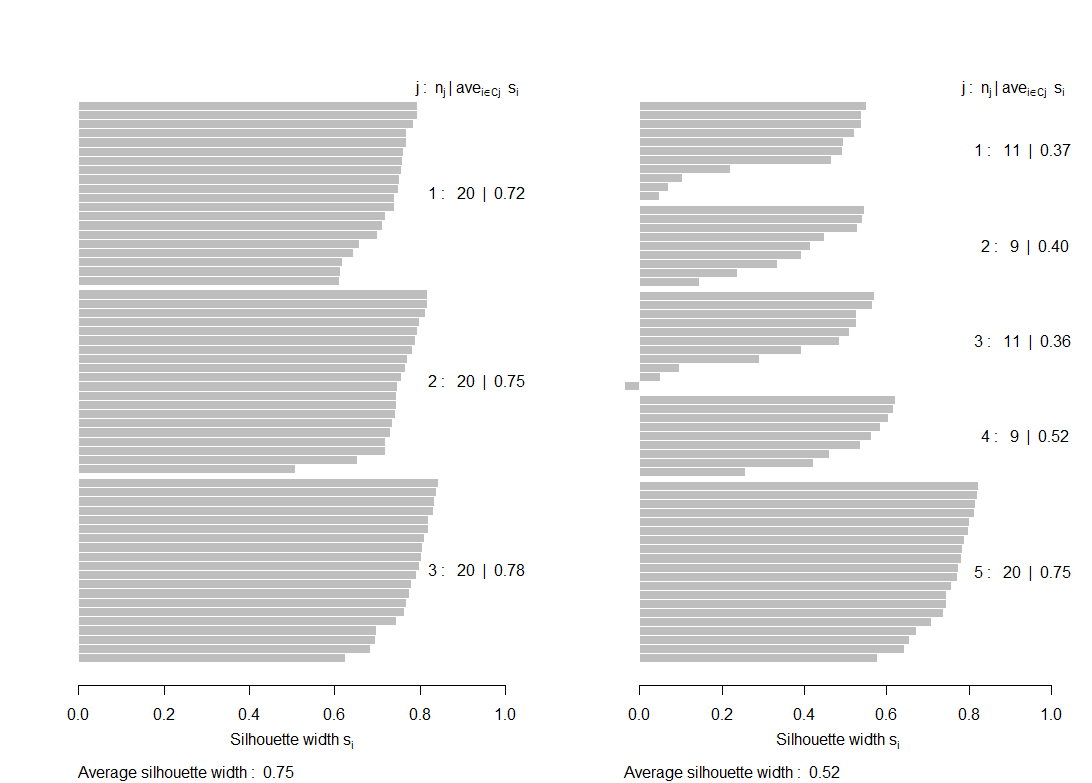
\includegraphics[width=\textwidth]{figures/chapter_k_means/silhouette}
	\caption{Left: silhouette plot for $k=3$; Right: silhouette plot for $k=5$}
	\label{fig:silhouette}
\end{figure}

Figure (\ref{fig:silhouette}) shows the silhouette plot for the sample data set with $k=3 \text{ and } 5$, respectively. Each silhouette plots shows on the right side the cluster name, the number of data points assigned to the cluster and the average silhouette width. In the right panel of figure (\ref{fig:silhouette}) cluster 1 consists of 11 data points and has a average silhouette width of $0.37$. In cluster 3, for example, two data points have a silhouette width $s(i)$ close to zero and one data point has a negative value for $s(i)$. Except for cluster 5, all other clusters include data points which have a small or even negative value for $s(i)$. At the bottom of each silhouette plot the average silhouette width for all data points is given. The silhouette plot with $k=3$ has much wider silhouettes compared to the plot with $k=5$ which is an indicator that only 3 clusters are present in the data. Similar plots for $k=2$ and $k=4$ also lead to the conclusion that the data consists of 3 natural clusters. If there are too many ($k > k_{true}$) or too few clusters ($k < k_{true}$) some of the cluster silhouettes will be much narrower compared to the others.  

\begin{remark}
A high average cluster silhouette width indicates that the cluster is well separated from other clusters and is not split up artificially. 
\end{remark}
\begin{remark}
It can be seen that artificial splits of clusters gets quite heavily penalizes by the silhouette coefficient. The average silhouette width drops from 0.75 to 0.52 if the number of cluster is increased from $k=3$ to $k=5$ as seen in figure (\ref{fig:silhouette}).
\end{remark}

%%%---------------------------------------------------------------------------------------------------------------------
%%%			Curse of dimensionality
%%%---------------------------------------------------------------------------------------------------------------------
\section{Curse of dimensionality}
After presenting two methods namely the elbow method and silhouette method which help identifying the correct number of clusters one should also be aware of phenomena that arise when analyzing data in high dimensional spaces. The `curse of dimensionality' is a term introduced by Richard Bellman \cite{bellman1961adaptive} to describe the rapid increase in volume and therefore the intractability of algorithms, when adding more dimensions of data to a mathematical space. Nowadays there are many different phenomenons referred to when talking about the curse of dimensionality but in the subsequent the focus is on distance functions as a measure of similarity. So far, all the methods presented are based extensively on the underlying distance functions used. To get a better understanding on the issue a simple example is given that helps to illustrate the problem.

\begin{example}\label{ex:curse_of_dimensionality}~
	\begin{enumerate}[label=(\roman*)]
		\item Imagine a line segment of length 1, and 10 data points which should represent the line. To capture the whole line segment one would distribute the points uniformly across the line. Therefore the line would be divided into 10 segments with length $\frac{1}{10}$ and the points are centered within these segments.
		\item By adding one dimension the line segment becomes a square segment with edge length 1. In order to represent the `same' space with a data point as in the one-dimensional case, the square would have to be divided into 100 smaller squares with an edge length of $\frac{1}{10}$ each. In the center of each of those square segments one data point is needed as a representative. A total of 100 data points are required to represent the square segment as exactly as the line segment. 
		\item By adding another dimension the square segment becomes a cube and 1000 points are needed. 
	\end{enumerate}
\end{example}

Example \ref{ex:curse_of_dimensionality} illustrates that as the number of dimensions increases the number of data points rises exponentially in order to represent the whole space properly. Thinking of insurance data, one can have data points with various numbers of dimensions ranging from just a few to several hundreds dimensions. Considering the fact that the cash flow projections of grouped policies should coincide over a 60 year horizon, it is easy to see that only 5 of these cash flow characteristics (e.g. premium, costs, ...)  result in data points with a dimension of 300. Of course, it is not advisable to include, over a period of 60 years, all cash flow variables in the grouping process, but it is much more difficult to find only those variables that are relevant for a major part of the results than including everything. For this reason, in practice more variables are often used than would actually be necessary. Another unintuitive fact one needs to be aware of is that the volume of a hypersphere inscribed into a hypercube is getting relatively smaller as the dimension increases. 

\begin{corollary}\label{cor:volume}
Let a hypersphere with radius $r$ and dimension $d$ be inscribed into a hypercube with edges of length $2r$. Then we get for the proportion of the volumes:
	\begin{equation*}
		\frac{V_{Sphere}}{V_{Cube}} =\frac{r^d\frac{\pi^{\frac{d}{2}}}{\Gamma(\frac{d}{2}+1)}}{(2r)^d} =\frac{\pi^{\frac{d}{2}}}{2^d\Gamma(\frac{d}{2}+1)} \rightarrow 0 \text{ as } d \rightarrow \infty
	\end{equation*}
\end{corollary}

\begin{remark}
Corollary \ref{cor:volume}  says that as dimension $d$ increases, more and more volume of the hypercube is outside the hypersphere. This means that under a uniform distribution most of the data points are located far from the center and thus close to an edge in a certain sense. 
\end{remark}

\begin{remark}
Some other examples why intuition fails in high dimensions are given in paragraph 6 of \cite{domingos2012few}.
\end{remark}

Not only do the data points move closer to the edge as the dimension $d$ of the data space increases, but the distance between the individual data points is becoming more and more similar. It can be shown (\cite{beyer1999nearest}) that under a broad set of conditions the distance to the nearest and to the farthest data point converges as dimensionality $d$ increases. Experimental results in \cite{beyer1999nearest} show that this effect can occur even for relatively low dimensional data with only 10 to 15 dimension. The fact that the distance to the farthest data point can get similar to the distance of the nearest data point makes clustering a hard job. The basic concept of $k$-means is to find, in the case of the Euclidean distance measure, spherically shaped clusters that have different characteristics. Therefore, data that is almost identical should not be clustered with a simple $k$-means algorithm without further analysis. Due to the fact that the $k$-means algorithm always returns a result even though there are obviously no clusters in the data because all data points are somehow similar, it is very difficult to determine whether $k$-means is a suitable tool for clustering or not. Situations in which all data points are similar and no cluster structure is present in the data are, as shown in the previous section, indicated by a low silhouette coefficient. When using the methods described in section \ref{sec:silhouette}, a silhouette plot with low silhouette coefficients for the clusters indicates that the clusters found by the algorithm are not well separated. Single clustering attempts can easily be verified by an visual inspection of plots described above. With an automated clustering approach, which is necessary for large insurance portfolios, visual control of the individual silhouette plots is not possible in most cases. In such cases, only a validation of the silhouette coefficient is feasible, but this leads ultimately to a situation where a clustering result is validated by a single value.
It is therefore advisable to use low-dimensional policy data sets or conduct a thorough analysis of the data to avoid situations where problems referred to as 'course of  dimensionality' occur. 







